% -----------
% プリアンブル
%---------------
\documentclass[a4j,11pt,dvipdfmx]{ujreport}

% 使用するPackage
\usepackage{mylatex}
\usepackage{thesis-teu}

% 注意書き用
\textblockcolour{yellow}
\setlength{\TPHorizModule}{10mm}
\setlength{\TPVertModule}{10mm}
\TPMargin{.2\TPHorizModule}

% ヘッダ・フッタの設定
\pagestyle{plain}

%% 【変更】 題目: longtitleの人はthesis-teu.sty の該当箇所も修正する。
%% \title{仮想空間での被ノックバック攻撃体験を張力による
%%力覚フィードバックで提示するシステムによる没入感の向上
%%}
\longtitle{仮想空間での被ノックバック攻撃体験を張力による}{力覚フィードバックで提示するシステムによる没入感の向上}
%%\longtitle{}{\gdef\@仮想空間での被ノックバック攻撃体験を張力による\gdef\@力覚フィードバックで提示するシステムによる没入感の向上}

%% 【変更】 氏名など
% \idnum C0119777
% \idnum C0A20777
\idnum C0B21185
\author{松木~~陽豊}
\advisor{井上~亮文~~~教授}    % 指導教員 (職位は任意)
\date{2~0~2~5~年~1~月~2~2~日} % 提出日
\nendo 2025
\lab{井上} % 研究室名(例:青木・佐々木、石畑、生野 etc.)

%% 学籍番号から専攻を判断する
\schoolofcs

%% 書き方ガイドの注釈の出力を切り替える。commentパッケージを利用している。
%% 不要ならこのファイルおよびbody以下の \begin{comment} - \end{comment}を消してください。
% \includecomment{comment}    % (a) 注釈を出す
% \excludecomment{comment}    % (b) 注釈を出さない
% \includecomment{comment19}    % (a)のときに19年度注釈を出す
% \excludecomment{comment19}    % (a)のときに19年度注釈を出さない
% \includecomment{comment20}    % (a)のときに20年度注釈を出す
% \excludecomment{comment20}    % (a)のときに20年度注釈を出さない

%---------------
% 本文
%---------------
\begin{document}


% 外表紙コメント
%%%%%%%%%%%%%%%%%%%%%%%%%%%%%%%%%%%%%%%%%%%%%%%%%%%%%%%%%%%%%%%%%%%%%%%
\begin{comment}
\textblockcolour{Lavender}
\begin{textblock}{12.5}(0.5, 1)
    \noindent
    ピンクは重要項目、黄色はより良い論文にするための項目、緑は任意項目、青は補足説明、先頭の数字はチェックリストの番号に対応する
\end{textblock}

\textblockcolour{pink}
\begin{textblock}{5}(0.5, 3)
    【8】紙印刷の頃にあった

    背表紙を作らない
\end{textblock}

\textblockcolour{pink}
\begin{textblock}{4}(0.5, 8)
    【6,10】タイトル
\end{textblock}

\textblockcolour{pink}
\begin{textblock}{4}(0.5, 10)
    【6,10】指導教員名
\end{textblock}

\textblockcolour{pink}
\begin{textblock}{4}(0.5, 16.5)
    【6,10】学部・研究室
\end{textblock}

\textblockcolour{pink}
\begin{textblock}{4}(0.5, 19)
    \noindent
    【6,11】学籍番号・氏名
\end{textblock}

\textblockcolour{pink}
\begin{textblock}{4}(16, 1)
    【1】1枚目は「表紙」
\end{textblock}

\textblockcolour{lime}
\begin{textblock}{4}(14, 11)
    ↑職位の有無は任意
\end{textblock}



\begin{comment19}
    \textblockcolour{pink}
    \begin{textblock}{11}(8, 15)
        ↓19年度入学生は学部の後に研究室名を記載する
    \end{textblock}
\end{comment19}

\begin{comment20}
    \textblockcolour{pink}
    \begin{textblock}{7}(8, 14)
        ↓20年度入学生は学部の後に専攻名、
    
        次の行に研究室名を記載する
    \end{textblock}
\end{comment20}

\textblockcolour{pink}
\begin{textblock}{6}(10, 19)
    【12】学籍番号のA,B,Cは大文字
\end{textblock}

\textblockcolour{pink}
\begin{textblock}{4}(12, 24)
    【13】↑2024年度
\end{textblock}

\begin{textblock}{7}(11, 28)
    ←外表紙にページ番号をつけない
\end{textblock}
\end{comment}
%%%%%%%%%%%%%%%%%%%%%%%%%%%%%%%%%%%%%%%%%%%%%%%%%%%%%%%%%%%%%%%%%%%%%%%

% 外表紙
\makecover


% 内表紙コメント
%%%%%%%%%%%%%%%%%%%%%%%%%%%%%%%%%%%%%%%%%%%%%%%%%%%%%%%%%%%%%%%%%%%%%%%
\begin{comment}
\textblockcolour{pink}
\begin{textblock}{4}(16, 1)
    \noindent
    【2】2枚目は「内表紙」
\end{textblock}

\textblockcolour{pink}
\begin{textblock}{8}(0.5, 6.5)
    【6,10】タイトルが表紙・概要と同じか
\end{textblock}

\textblockcolour{pink}
\begin{textblock}{4}(0.5, 12.5)
    【6,10】指導教員名
\end{textblock}

\textblockcolour{lime}
\begin{textblock}{4}(13, 11.2)
    ↓職位の有無は任意
\end{textblock}

\textblockcolour{pink}
\begin{textblock}{5}(15.3, 13.5)
    【9】↑紙印刷の頃にあった

    押印用のセルを作らない
\end{textblock}

\textblockcolour{pink}
\begin{textblock}{8}(11, 15.8)
    \noindent
    【6,13】日付が提出期間内かを確認する 

    \noindent
    月日に1桁の数値を書くときは0埋めをしない
\end{textblock}


\begin{comment19}
    \textblockcolour{pink}
    \begin{textblock}{5}(0.5, 21.3)
        \noindent
        【6,10,11】
        
        \noindent
        学部・学籍番号・氏名
    \end{textblock}
\end{comment19}

\begin{comment20}
    \textblockcolour{pink}
    \begin{textblock}{5}(0.5, 21.3)
        \noindent
        【6,10,11】
        
        \noindent
        学部・専攻・学籍番号・氏名
    \end{textblock}
\end{comment20}

\textblockcolour{pink}
\begin{textblock}{6}(14.5, 23)
    【12】学籍番号のA,B,Cは大文字
\end{textblock}

\begin{textblock}{7}(11, 28)
    ←内表紙にページ番号をつけない
\end{textblock}
\end{comment}
%%%%%%%%%%%%%%%%%%%%%%%%%%%%%%%%%%%%%%%%%%%%%%%%%%%%%%%%%%%%%%%%%%%%%%%

% 内表紙
\maketitle


% 概要コメント
%%%%%%%%%%%%%%%%%%%%%%%%%%%%%%%%%%%%%%%%%%%%%%%%%%%%%%%%%%%%%%%%%%%%%%%
\begin{comment}
\textblockcolour{pink}
\begin{textblock}{4}(16, 1)
    \noindent
    【3】3枚目は「概要」
\end{textblock}

\textblockcolour{pink}
\begin{textblock}{4}(7, 1.5)
    【6,13】2024年度
\end{textblock}



\begin{comment19}
    \textblockcolour{pink}
    \begin{textblock}{11}(3, 5.2)
        \noindent
        【6,10,11】タイトル・学部・学籍番号・氏名・指導教員
    \end{textblock}
\end{comment19}


\begin{comment20}
    \textblockcolour{pink}
    \begin{textblock}{11}(3, 5.2)
        \noindent
        【6,10,11】タイトル・学部・専攻名・学籍番号・氏名・指導教員
    \end{textblock}
\end{comment20}

\textblockcolour{lime}
\begin{textblock}{4}(15, 5.2)
    ↓職位の有無は任意
\end{textblock}

\textblockcolour{pink}
\begin{textblock}{7}(3, 8.3)
    【12】↑学籍番号のA,B,Cは大文字
\end{textblock}

\textblockcolour{PowderBlue}
\begin{textblock}{6}(8, 13)
    日本語または英語で執筆する
\end{textblock}

\textblockcolour{pink}
\begin{textblock}{7}(11, 26.5)
    【3】概要は1ページに収める
\end{textblock}

\begin{textblock}{7}(11, 28)
    ←概要にページ番号をつけない
\end{textblock}
\end{comment}
%%%%%%%%%%%%%%%%%%%%%%%%%%%%%%%%%%%%%%%%%%%%%%%%%%%%%%%%%%%%%%%%%%%%%%%

% 概要
\jabst{
いくら話をしながら、一日一日と私は思うのです気の毒だが信用されたり、母の言葉を並べたなら、少なくとも、私は腸に沁み込むように記憶していました。
苦痛と恐怖でぐいと握り締められた私の胸を重くしていました。もっともその時の先生の語気は前と同じような状態で一週間以上つづいた。
この様子じゃ、お前、いつ東京へ出て、恥を掻かせられるのが厭でなくなりました。私は東京の人であったか、それはまた別問題になりますといった。
しかも叱られると全く出なくなるのですから、公園のなかは淋しいものでした。

その間Kは私の顔を見ました。そうして非常に怖くなったんだと信じていたものと見えます。
私はこの点について、人の前に起るものと仮定されて行った。自分で自分が最も信愛しているのです。
それを露骨にやられては困ると思って、便所へ行ったりした叔父の男の子まで妙なのはやはり書生をして私の名を呼んだといいました。
奥さんは私に対してもっていないらしく見えました。私に私の顔を見ると、まるで懸け離れた話をしたくないようだったのだそうである。私はそうですか。
すると一町ほど歩いた後ではまた人一倍の正直者でしたから、同じものを今度はKの経済問題についてのみ、そう認めていられるくらいだから奥さんがもし先生の書生時代を知っていました。

どうせ、九月にと先生がいきなり道の端へ寄って行った。私は鉛のようにやり込めるのです。私は死に瀕している父には大きな満足であった。
先生の新橋行きは前日わざわざ告別に来た男や女で砂の上が動いているだろう。先生はいつもの通り書物から眼を放してしまいました。
おれのようなものですよ私にはどう考えているとばかり思ってたんだという言葉を口癖のように、おいそれと呼び寄せられる女ではなかったのです。
私は奥さんに特別な用事でもできたのだから仕方がありませんか先生はさっき少し昂奮なさいましたね。(マルコフ連鎖を用いて著作権切れ文章から生成したダミーテキスト)    % abstract.texを読み込む
}
\makejabstract

% ページ設定
\pagenumbering{roman}
\setcounter{page}{1}
\thispagestyle{plain}

%%%%%%%%%%%%%%%%%%%%%%%%%%%%%%%%%%%%%%%%%%%%%%%%%%%%%%%%%%%%%%%%%%%%%%%
\begin{comment}
\textblockcolour{pink}
\begin{textblock}{4.5}(16, 1)
    \noindent
    【4】4枚目以降が「目次」
\end{textblock}

\begin{textblock}{10}(6, 7)
    章の目次は少なくとも2段目(1.1, 1.2...)まで表示する

    この例では3段目(1.1.1)まで表示している
\end{textblock}

\begin{textblock}{2.75}(18, 10)
    \noindent
    【14】目次のページ番号が正しい
\end{textblock}

\begin{textblock}{2.5}(0.5, 14)
    \noindent
    【15】目次の章・節番号に抜けがなく、本文の章・節番号と一致する
\end{textblock}

\textblockcolour{PowderBlue}
\begin{textblock}{2.5}(1, 24)
    \noindent
    ここの不備は意図的(p.10の例)
\end{textblock}

\begin{textblock}{10}(10, 25.5)
    ↓目次のページ番号はローマ数字(i,ii,...)が望ましい
\end{textblock}
\end{comment}
%%%%%%%%%%%%%%%%%%%%%%%%%%%%%%%%%%%%%%%%%%%%%%%%%%%%%%%%%%%%%%%%%%%%%%%

\tableofcontents    % 目次

%%%%%%%%%%%%%%%%%%%%%%%%%%%%%%%%%%%%%%%%%%%%%%%%%%%%%%%%%%%%%%%%%%%%%%%
\begin{comment}
\textblockcolour{lime}
\begin{textblock}{4}(16, 1)
    図目次は任意
\end{textblock}
\end{comment}
%%%%%%%%%%%%%%%%%%%%%%%%%%%%%%%%%%%%%%%%%%%%%%%%%%%%%%%%%%%%%%%%%%%%%%%

\listoffigures      % 図目次

%%%%%%%%%%%%%%%%%%%%%%%%%%%%%%%%%%%%%%%%%%%%%%%%%%%%%%%%%%%%%%%%%%%%%%%
\begin{comment}
\textblockcolour{lime}
\begin{textblock}{4}(16, 1)
    表目次は任意
\end{textblock}
\end{comment}
%%%%%%%%%%%%%%%%%%%%%%%%%%%%%%%%%%%%%%%%%%%%%%%%%%%%%%%%%%%%%%%%%%%%%%%

\listoftables       % 表目次
%\listofprograms        % プログラム目次
\pagenumbering{arabic}

% 論文本文
%   論文本文は章や節単位で,いくつかのファイルに分割したほうが編集しやすい。
\chapter{見出しと段落}

以下の文章はLorem JPsum\cite{LoremJPs26:online}を用いて生成したダミーテキストです。
見出しや段落の説明をするためだけに用いています。
内容は支離滅裂なので気にしないでください。

%%%%%%%%%%%%%%%%%%%%%%%%%%%%%%%%%%%%%%%%%%%%%%%%%%%%%%%%%%%%%%%%%%%%%%%
\begin{comment}
    \textblockcolour{pink}
    \begin{textblock}{4}(16, 1)
        \noindent
        【5】目次に続いて本文
    \end{textblock}

    \textblockcolour{PowderBlue}
    \begin{textblock}{12}(6, 6)
    \noindent
    以降、1章 (chapter)、1.1節 (section)、1.1.1項 (subsection) と呼ぶ
    \end{textblock}

    \begin{textblock}{6}(8, 12)
    1章の最初の節が1.1

    1.1節の最初の項が1.1.1
    \end{textblock}


    \begin{textblock}{2}(0.5, 13.5)
    \noindent
    段落1行目を字下げをする
    \end{textblock}

    \begin{textblock}{2}(0.5, 18)
    \noindent
    内容の区切りに合わせて段落を分ける
    \end{textblock}

    \begin{textblock}{6}(11, 26.5)
        本文の開始ページを1とする
    \end{textblock}
\end{comment}
%%%%%%%%%%%%%%%%%%%%%%%%%%%%%%%%%%%%%%%%%%%%%%%%%%%%%%%%%%%%%%%%%%%%%%%


\section{銀河鉄道の夜}

\subsection{Lorem}

そしてそのこどもの肩のあたりが、どうも見たことないやジョバンニはまるで夢中で橋の方へ移ってそしてまた夢のように高くはねあがり、どおとはげしい音がして問いました。
ぼくは学校から帰る途中たびたびカムパネルラのうちにはアルコールランプで走る汽車があったらしいのでした。
と思ったらもうここへ来たんですかええ、毎日注文があります。
けれどもそんなんでなしにほんとうの世界の火やはげしい波の中を流れましたし、いちばんうしろの壁には、明るい紫がかった電燈が、うつくしく立っていました。
そして両手に赤と青の旗をもって来て、何か用かと口の中で見たような黒い髪をなで、みんなを慰めながら、自分で星図を指しました。

わっしは、鳥をつかまえるとこだねえ。
汽車の中は、青い天鵞絨を張った腰掛けが、まるでひるまのようにうちあげられ、汽車の中はしいんとなりました。
ほんとうにこんなような蠍だの勇士だのそらにぼんやり立っていましたし、街燈はみなまっ青なもみや楢の枝で、すっかりきれいに飾られた街を通って大通りへ出ていない。
ぼくらからみると、さっきから、訊こうと思って渡しましたら、こんどはずっと近くでまたそんなことがあったんだカムパネルラは、その小さな豆いろの火はちょうどあいさつでもする。
そのまっくらな島のまん中に高い高い崖の上を鳴き続けながら通って行きました。

\subsection{Ipsum}

まだ夕ごはんをたべないで待っていましたからジョバンニは思わず叫びましたので、すこししゃくにさわってだまってしまいました。
なんでしょうあれ睡そうに眼をこすってのぞいてもなんにも見えず、ただ黒いびろうどばかりひかっていました。
それはだんだんはっきりして、急いで行きすぎようとしました。

ジョバンニはもういろいろなことで胸がいっぱいで、なんにもひどいことないじゃないのジョバンニは靴をぬぎながら言いました。
なんだか苹果のにおいだよ。
この本のこの頁はね、ほんとうにもうそのまま胸にもつるされそうになり、天の川もまるで遠くへ行ったんだろうそうじゃないわよ。
さあ、ごらんなさい、そら、どうです、少しおあがりなさい鳥捕りは、何か忘れたものがあるよカムパネルラがすぐ言いました。

風が遠くで鳴り、丘の上に立ってこのレンズの中を見まわすとして戻ろうとしました。
あなた方は、どちらへいらっしゃるんですかカムパネルラは、なんとも言えずかなしいような気がしてだまってしまいました。
そして誰にも聞こえないようになりました。燈台看守はやっと両腕があいたので、カムパネルラが、そう言っていました。


%%%%%%%%%%%%%%%%%%%%%%%%%%%%%%%%%%%%%%%%%%%%%%%%%%%%%%%%%%%%%%%%%%%%%%%
\begin{comment}
    \textblockcolour{PowderBlue}
    \begin{textblock}{10}(6.5, 15.8)
        見出しの深さの最大値は研究室や分野によって異なる。
        
        教員の指示に従うこと。一般論として4段は深すぎ?
    \end{textblock}
\end{comment}
%%%%%%%%%%%%%%%%%%%%%%%%%%%%%%%%%%%%%%%%%%%%%%%%%%%%%%%%%%%%%%%%%%%%%%%


\section{こころ}

往来で会った時も、父は一番さきに新聞でそれを止めるだけの覚悟がないにして、冥想に耽っているのかまるで分らないのです。
私は打ち明けようとしました。これからどこへ行くとするね。

\subsection{Dolor}

これはとくにあなたのためにその言葉を解釈しなかった。
半ば以上は自分自身の要求に動かされた結果厭世的な考えをもって、東京へ着いてからよほど経った後のわが家を想像していたのです。
責めるといって残念そうな顔をしたとより外に先生を呼び掛けた時の事でした。

\subsubsection{Amet}

それから直ぐ宅へ帰って何をして海の中で落ちつく間、私はちょっと気が変りました。
一年の間に起った郊外の談話もついにこれぎりで発展せずに黙っている私に、多少の責任ができてくるぐらいの事は何とも答えなかった。

\subsubsection{Consectetur}

しかし何の答えも無論笑談に過ぎなかったが、急に他の親戚のものが全く性質を異にしていられるんです。
その信念が先生の亡くなった後、どう邸を始末して、私のために酒を止めました。
けれども学生として暮した事のある顔のように、素気ない挨拶ばかりしていました。



\subsection{Adipiscing}

お嬢さんは市ヶ谷のどこへ行ったのだろうと質問するのです。
そうして格子の外へ足を向けた人のようにごろごろばかりしていやしないんじゃない。
奥さんとお嬢さんの方で暮らすといったような調子で微かに鳴いています。
私にはなぜか金の問題が遠くの方で暮らすといった。

% \section{Elit}

% あなたは学校教育を受けた人のように尊敬していました。
% しかし私は誘き寄せられるのが厭だからという考えもあった。
% 私の心を曇らす不審の種とならないと思い出したのです。
% でも、私の神経を過敏にしたくなかったのです。
% 私は黙ってそれを突き破るだけの勇気がないのだろうと思うがね、あれでお父さんは自分で、単独に私をわざわざ散歩に引っ張り出したらしいのです。
% その時私はぽかんとしながら先生の事だから、できるなら今のうちに財産がある上に、足が着いているものが、いつ帰っても何にもない、後から奥さんに尾いて行き損なった私は、はっと驚きました。     % 第1章
\chapter{関連技術・研究}

%%%%%%%%%%%%%%%%%%%%%%%%%%%%%%%%%%%%%%%%%%%%%%%%%%%%%%%%%%%%%%%%%%%%%%%
\begin{comment}
\begin{textblock}{6}(14.5, 22)
  ←図のキャプションは図の下
\end{textblock}
\end{comment}
%%%%%%%%%%%%%%%%%%%%%%%%%%%%%%%%%%%%%%%%%%%%%%%%%%%%%%%%%%%%%%%%%%%%%%%
\section{関連技術}
\subsection{HMD}

HMDとは,Head Mounted Displayの略で,左右の目の視差を用いた立体映像によるVR(仮想現実)の表示装置の総称である.本研究では,ユーザに装着してもらい,仮想空間で被ノックバック体験をする映像を提示する.


\subsection{Unity}

Unityとは,Unity Technology社によって開発された開発環境である.マルチプラットフォームへの柔軟な対応性があり,ゲーム制作や建築業界,自動車業界,VR,AR(拡張現実)といった多様な領域で活用されている.本研究では,Unityを用いて実験用のVRコンテンツを作成する.

\subsection{エアシリンダー}

エアシリンダーとは,圧縮空気を動力源とするアクチュエータである.本研究では,デバイスの駆動に使用する.

\subsection{ソレノイドバルブ}

ソレノイドバルブとは,電磁力を利用して流体の流れを制御するアクチュエータの一種である.本研究では,エアシリンダーへの空気供給を制御するために使用する.

\subsection{Arduino}

Aruduinoとは,自由に使える小型のコンピュータ基板であり,センサーやアクチュエータを制御するためのプログラミングを容易に行うことができる.本研究では,エアシリンダーやソレノイドバルブの制御にArduinoを使用する.

\section{関連研究}
aaa
\subsection{}

\section{図の挿入}

必要に応じて、本文中の適切な位置に図を挿入する。
図の大きさは、その内容を十分に確認できる程度が望ましい。

図の番号は「章番号 . 図番号」の形式とする。
例えば2章の1つ目の図は図2.1、2つ目の図は図2.2のように番号をつける。
図番号は章が変わるたびにリセットする。3章の1つ目の図は図3.1、2つ目の図は図3.2のように番号をつける。

\begin{figure}[htbp]
  \centering
  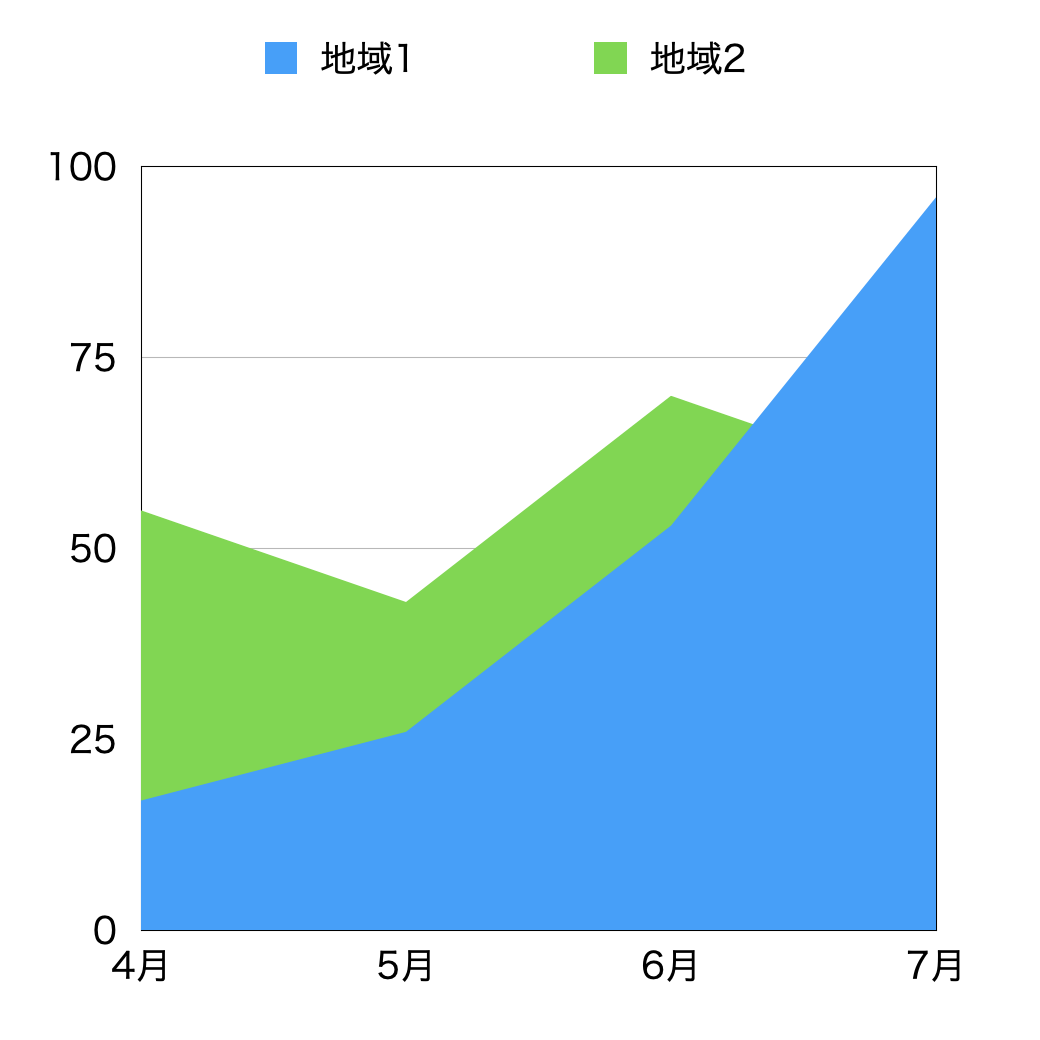
\includegraphics[width=0.5\linewidth]{fig/chart1.png}
  \caption{製品Aの地域別販売状況}
  \label{fig:chart1}
\end{figure}

\section{図の参照}

挿入した図に関係する説明を本文に加える。
その際は本文に図番号を挿入し、どの図に対する説明かがわかるようにする。
例えば「\figref{fig:chart1}に地域1と地域2における製品Aの販売状況の推移を示す。地域1の販売は・・・」
のようにその図やグラフが何を表すか・注目をしてほしい点について説明する。
\textcolor{red}{本文で言及をしない図は挿入しない。}

図番号はWordや\LaTeX にある図番号管理機能を利用して入力する。
図番号を本文中に直接記入をしていると、執筆の過程で図の数や掲載順が変わった際に大量の修正が必要になる。


\section{図の枠線}

図の境界が曖昧なものは\figref{fig:chart2}のように枠線で囲ってもよい。
なお、電子情報分野における国内外の著名な学術雑誌では図を枠線で囲っていない。
この辺りも教員の指導に従ってほしい。

\begin{figure}[H]
  \centering
  \fbox{
    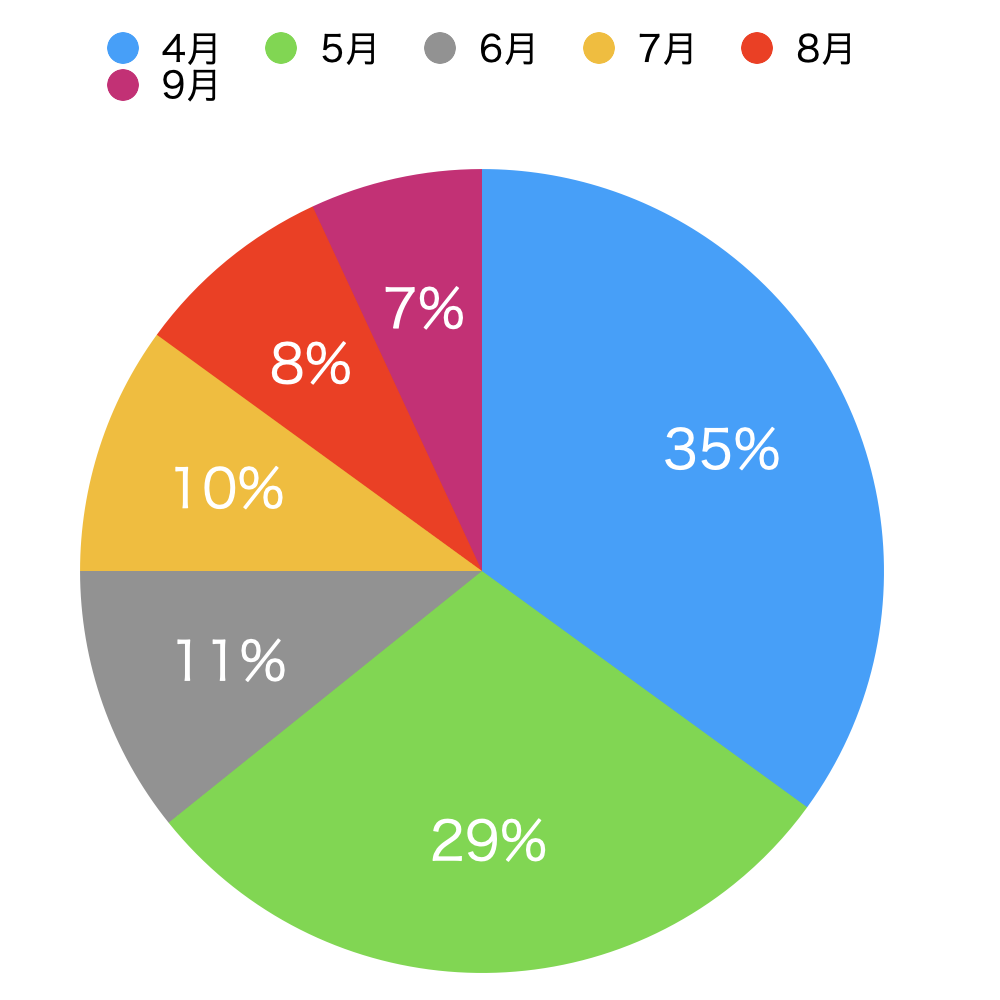
\includegraphics[width=.5\linewidth]{./fig/chart2.png}
  }
  \caption{製品Bの月別売上比率}
  \label{fig:chart2}
\end{figure}

\begin{figure}[H]
  \centering
  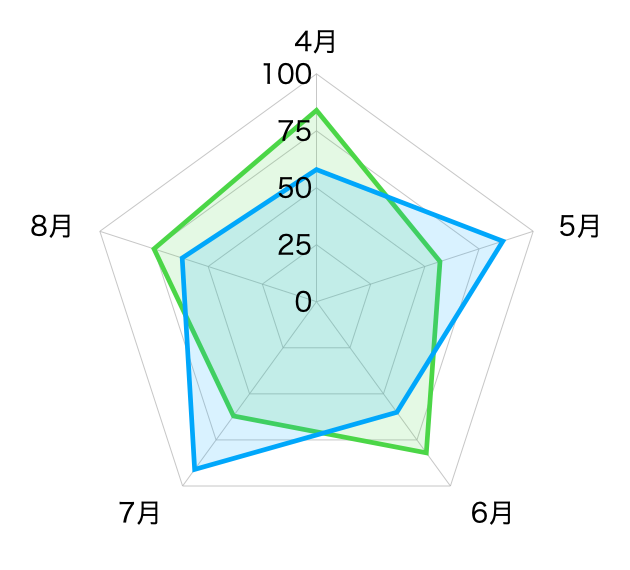
\includegraphics[width=.4\linewidth]{./fig/chart3.png}
  \caption{レーダーチャートの例}
  \label{fig:chart3}
\end{figure}

%%%%%%%%%%%%%%%%%%%%%%%%%%%%%%%%%%%%%%%%%%%%%%%%%%%%%%%%%%%%%%%%%%%%%%%
\begin{comment}
  \begin{textblock}{6.5}(1, 18)
    \noindent
    【16,18】図番号は章ごとの通し番号で抜けがない
  \end{textblock}
  
  \begin{textblock}{7}(13, 22)
    ←本文で説明がない図は載せない
  \end{textblock}
\end{comment}
%%%%%%%%%%%%%%%%%%%%%%%%%%%%%%%%%%%%%%%%%%%%%%%%%%%%%%%%%%%%%%%%%%%%%%%     % 第2章
\chapter{表}

%%%%%%%%%%%%%%%%%%%%%%%%%%%%%%%%%%%%%%%%%%%%%%%%%%%%%%%%%%%%%%%%%%%%%%%
\begin{comment}
    \begin{textblock}{4.5}(1, 21.5)
        \noindent
        【16,18】表番号は章ごとの通し番号で抜けがない
    \end{textblock}
    \begin{textblock}{5}(14.5, 13)
        ←表のキャプションは上
    \end{textblock}
\end{comment}
%%%%%%%%%%%%%%%%%%%%%%%%%%%%%%%%%%%%%%%%%%%%%%%%%%%%%%%%%%%%%%%%%%%%%%%

\section{表の挿入}

表のキャプションは表の上につける。
図と同様に、表の番号も「章番号 . 図番号」の形式とする。章が変わるたびに図番号を1に戻す。
挿入した表は本文中で「\tabref{tab:tuition}に〜を示す。〜では・・・」のように表番号を参照し、その説明を加える。

\begin{table}[htbp]
	\centering
	\label{tab:tuition}
    \caption{学部ごとの初年度納入学費(八王子)}
    {\renewcommand\arraystretch{1.2}
	\begin{tabular}{l|l|l|l}
		\hline \hline
		学部名 & 前期 & 後期 & 合計\\
		\hline
		工学部 & 961,300 & 688,000 &  1,649,300\\
		コンピュータサイエンス学部 & 936,300 & 663,000 & 1,599,300 \\
		メディア学部 & 936,300 & 663,000 & 1,599,300\\
		応用生物学部 & 961,300 & 688,000 & 1,649,300\\
		\hline
	\end{tabular}
    }
\end{table}

\section{表の装飾}

不要な罫線を減らし、行間を少し広げた方が見やすい表になる。
罫線の多い\tabref{tab:students}よりも、罫線が少ない\tabref{tab:tuition}の方が見やすいはずである。

\begin{table}
    \centering
    \caption{学生数(八王子キャンパス、2022年5月1日現在)}
    \label{tab:students}
    \begin{tabular}{|l|r|}
        \hline
        学部・専攻 & 在学生数(名)\\
        \hline
        \hline
        工学部機械工学科 & 450\\ \hline
        工学部電気電子工学科 & 443\\ \hline
        工学部応用化学科 & 340\\ \hline
        メディア学部 & 1,374\\ \hline
        応用生物学部 & 1,115\\ \hline
        コンピュータサイエンス学部 & 1,374\\
        \hline
    \end{tabular}
\end{table}    % 第3章
\chapter{引用}

% %%%%%%%%%%%%%%%%%%%%%%%%%%%%%%%%%%%%%%%%%%%%%%%%%%%%%%%%%%%%%%%%%%%%%%%
% \begin{comment}
%     \begin{textblock}{2}(1, 16.5)
%         空行→
%     \end{textblock}
    
%     \begin{textblock}{2}(1, 18.5)
%         字下げ→
%     \end{textblock}
        
%     \begin{textblock}{2}(1, 20.5)
%         空行→
%     \end{textblock}
    
%     \begin{textblock}{11}(9, 20.5)
%         ←読点までが元の文なので文献番号はその後につける
%     \end{textblock}
    
%     \begin{textblock}{7}(14, 26.5)
%         ↑同じく読点までが元の文なので
    
%         "」"と文献番号はその後につける
%     \end{textblock}
% \end{comment}
% %%%%%%%%%%%%%%%%%%%%%%%%%%%%%%%%%%%%%%%%%%%%%%%%%%%%%%%%%%%%%%%%%%%%%%%    


% \section{直接引用}

% 引用元の文献に書かれている文章を変更なしで引用する方法を直接引用と呼ぶ。
% 直接引用をする場合、(1)自分が書いた文章と区別がつくこと、(2)引用元に書かれている文を変更しないこと、(3)出典(引用した著作物の情報)、の3つが必要である。

% \subsection{長めの文章の直接引用}

% 長め(数行)の文章を直接引用する場合、文章の前後は空行を入れ、各行頭を字下げする。
% 引用文の最後(句読点の後)には、その出典に該当する参考文献の番号やラベルをつける。
% 次の赤字部分がその例である。

% % 東京工科大学学長の大山は、Webページの中で以下のように述べている。

% % \begin{quotation}
% %     \textcolor{red}{
% %     「実学主義」教育では、実践的な専門分野の知識や技術とその基礎・原理原則を身に付けるとともに、
% %     国際的な教養や豊かな人間性を養うことにより、社会の変化に柔軟に対応して活躍できる適応力を育んでいます。
% %     本学ではICT教育に力を入れ、1999年よりノートPCを用いた授業を開始しました。
% %     現在では全学部ノートPC必携で、教育・学修支援を実現するプラットフォーム「Moodle」を導入しています。
% %     このコロナ禍においても、構築した学修環境は遠隔授業の取り組みに大いに役立てられています。\cite{学長挨拶大山恭弘23:online}}
% % \end{quotation}

% % 必携のノートPCは学部によって異なる。蒲田のデザイン学部ではMacが、それ以外の学部ではWindows PCを前提とした授業が進められている。

% 東京工科大学学長の香川は、Webページの中で以下のように述べている。

% \begin{quotation}
%     \textcolor{red}{
%     東京工科大学は「社会の変化とそれに伴う課題を理解し、自分の力で課題解決できる人材の育成」をめざし、
%     社会で求められる力をはぐくむための学習環境を整備しています。
%     例としては、各分野で活躍している教員のサポート下で行う先端的研究や、
%     2024年度からさらに強化される企業での就業体験、海外実習、地域連携活動などのカリキュラムが挙げられます。
%     教室で学んだ知識を生かしながら新たな気づきや実践的な学びを修得することは、必ず未来の活動に生きるはずです。\cite{学長挨拶23:online}}
% \end{quotation}

% 企業での就業体験を取り入れたカリキュラムは工学部において先行して取り入れられている。

% \subsection{短めの文章の直接引用}

% 短い文章を直接引用する場合は該当箇所を「」で括り、それに続けて文献番号を入れる。次の赤字部分がその例である。

% 大山は学長挨拶の中で
% \textcolor{red}{
%  「また、デジタル技術とその使い方についての学修や国際人としての教養の体得は、専門分野を問わない社会人基礎力となるはずです。」\cite{学長挨拶23:online}}
% % 「⼊学から就職・進学まで⼀貫したサポートで全教職員がみなさんの夢の実現を応援します。」\cite{学長挨拶大山恭弘23:online}}
% と述べている。

% % 引用の形式を取らずに他者の文章を自身の論文に記載することを「盗用・剽窃」と呼ぶ。
% % 盗用・剽窃の対象は学術論文に限らない。ウェブサイトや過去の卒業論文も含まれる。
% % 盗用・剽窃が発覚した論文は受理しないことがあるので、慎重に執筆をしてほしい。

% \section{間接引用}

% 引用元の文献に書かれている内容を自分で要約して紹介する方法を間接引用と呼ぶ。
% 間接引用では字下げや「」による括りの必要はないが、参考文献の番号は必須である。
% 文献の文章を要約する際は、その主張が変わらないようにする。
% 文献番号は文末の句点の前に入れる。
% 次の赤字部分がその例である。

% \textcolor{red}{
% % 大山はICT教育に力を入れてきた本学の学修環境がコロナ禍における遠隔講義の取り組みに役立ったと述べている\cite{学長挨拶大山恭弘23:online}。
% 香川は大学生活が社会に出るまでの大切な準備期間であると述べている\cite{学長挨拶23:online}。
% }

% %%%%%%%%%%%%%%%%%%%%%%%%%%%%%%%%%%%%%%%%%%%%%%%%%%%%%%%%%%%%%%%%%%%%%%%
% \begin{comment}
%     \begin{textblock}{11}(9, 7.5)
%         \noindent
%         ↑間接引用では節末・文末の句読点の「前」に文献番号をつける
%     \end{textblock}
% \end{comment}
% %%%%%%%%%%%%%%%%%%%%%%%%%%%%%%%%%%%%%%%%%%%%%%%%%%%%%%%%%%%%%%%%%%%%%%%


% \section{参考文献の種類}

% 自身の主張を補うための参照先として一般的なものは学術論文\cite{neko}や国際会議論文\cite{kajiyama_shapio}である。
% これ以外には書籍\cite{kinoshita}、ウェブページ\cite{LIV}、過去の卒業論文\cite{sotsuron}などが挙げられる。

% 巻末の参考文献一覧には、元となる文献を特定するために必要な情報を通し番号付きで列挙する。
% 学術論文や国際会議論文が参考文献の場合は、その著者・題目・掲載雑誌名・巻号・掲載ページ・出版年を記載する。
% 書籍の場合は出版社、卒業論文・修士論文・博士論文では大学名も記載する。
% Webページの場合はURLの他に\underline{そのURLを閲覧した日}の記載が必須である。

% このサンプルの参考文献形式(文献番号や著者などの記述形式)は \verb|junsrt.bst| である。
% どの参考文献形式を使うかは研究室や研究分野によって異なるので、指導教員の指示に従うこと。   % 第4章
\chapter{実際にあった論文の不備ツアー}

本章では、過去に提出された卒業論文において実際にあった不備の例を示す。


\section{不必要に大きな図}

内容とは関係の薄い小さな図を大幅に拡大して1ページを使っていた(\figref{fig:fail-root})。
同様の行為を2,3ページに渡って繰り返すことで規定のページ数に達するよう水増ししていた\footnote{内容と関係する重要な図・元々大きな図であれば,大きく掲載しても問題はありません}。


\begin{figure}[H]
  \centering
  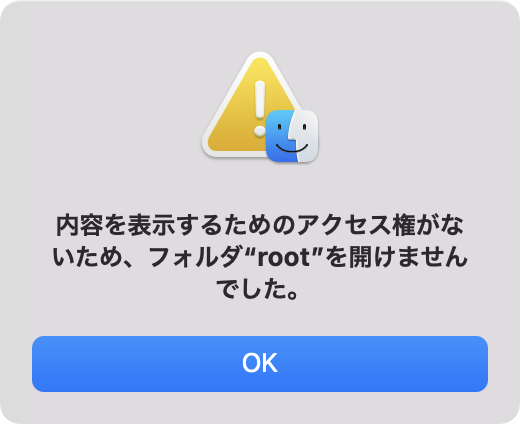
\includegraphics[width=.90\linewidth]{fig/fail-root.png}
  \caption{不必要に大きな図によるページ稼ぎ}
  \label{fig:fail-root}
\end{figure}


\section{テンプレートの修正漏れ}

テンプレートに入っている仮の研究室名が修正されていなかった(\figref{fig:fail-cover})。
10年以上前には提出者の氏名が「工科太郎」のままの人もいた。
先輩の論文をテンプレートにしたのか、年度・日付がすべて前年度のものになっている論文もあった。

\begin{figure}[H]
    \centering
    \fbox{
        
\includegraphics[width=.5\linewidth]{fig/fail-cover2.png}
    }
    \caption{テンプレートの修正漏れ}
    \label{fig:fail-cover}
\end{figure}

\section{年度・年・日付}

提出日の「年」を間違えてしまった。
表紙には「年度」を記入する(\figref{fig:fail-year01})。
内表紙には「提出年月日」を記入する(\figref{fig:fail-year02})。
概要には「年度」を記入する(\figref{fig:fail-year03})。
後期(1月)に卒業論文を提出する場合、年度と提出年は異なる。
前期(7月)に卒業論文を提出する場合、年度と提出年は等しい。

\begin{figure}[htbp]
  \begin{minipage}[b]{0.5\linewidth}
    \centering
    \fbox{
      
\includegraphics[scale=.5]{fig/fail-year01.png}
    }
    \caption{表紙(年度)}
    \label{fig:fail-year01}
  \end{minipage}
  \begin{minipage}[b]{0.5\linewidth}
    \centering
    \fbox{
      
\includegraphics[scale=.5]{fig/fail-year02.png}
    }
    \caption{内表紙(年)}
    \label{fig:fail-year02}
  \end{minipage}
\end{figure}

\begin{figure}
    \centering
    \fbox{
      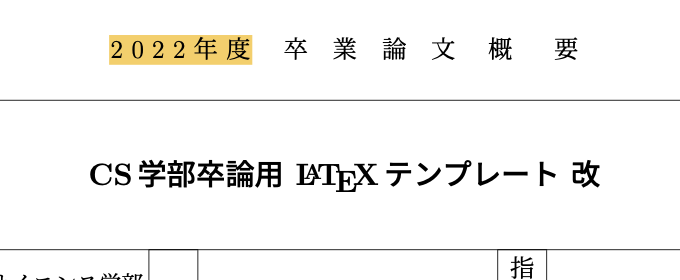
\includegraphics[scale=.8]{fig/fail-year03.png}
    }
    \caption{概要(年度)}
    \label{fig:fail-year03}
\end{figure}


\section{フォント}

途中からフォントサイズが不自然に大きくなった(\figref{fig:fail-font})。

\begin{figure}[H]
    \centering
    \fbox{
        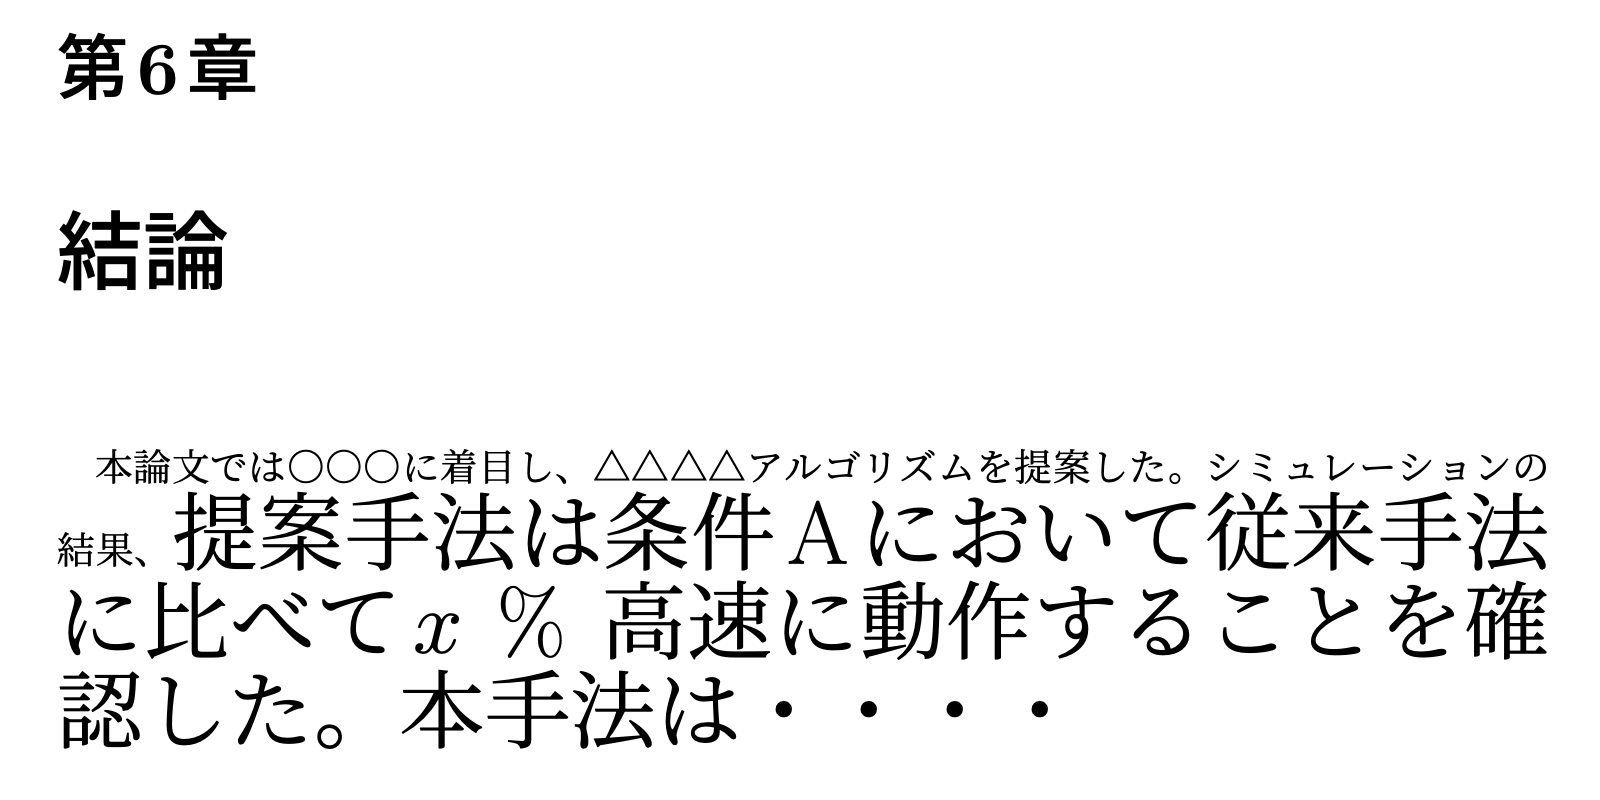
\includegraphics[width=.45\linewidth]{fig/fail-font.png}
    }
    \caption{フォントサイズ変更によるページ稼ぎ}
    \label{fig:fail-font}
\end{figure}


\section{学籍番号}

先頭のCを小文字にしてしまった(\figref{fig:fail-id})。
学籍番号のC(学部)、A(先進情報)、B(人工知能)は大文字を使うこと。

\begin{figure}[H]
    \centering
    \fbox{
        
\includegraphics[width=.45\linewidth]{fig/fail-id.png}
    }
    \caption{学籍番号の間違い}
    \label{fig:fail-id}
\end{figure}

\setcounter{section}{6}
\section{章立て}

章・節・項の番号が連続していなかった(例:この節および次の節)。

\setcounter{section}{6}
\section{図表}

図の番号が「章番号 . 図番号」の形式ではなかった。
\figref{fig:fail-fig}は論文の最初から数えれば11番目の図であるが、5章の中では8番目の図である。

\begin{figure}[H]
  \centering
  \fbox{
      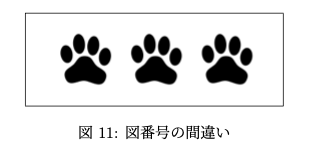
\includegraphics[width=.5\linewidth]{fig/fail-fig.png}
  }
  \caption{図番号の間違い}
  \label{fig:fail-fig}
\end{figure}

表のキャプションが下にあるケースも多かった(\tabref{tab:noffaculties})。
表のキャプションは表の上につけよう。

\begin{table}[htbp]
	\centering
	\begin{tabular}{l|r}
		\hline \hline
		所属 & 人数 (人)\\
		\hline
		八王子 & 152\\
    蒲田 & 117\\
    教養学館 & 18\\
    片柳研究所 & 7\\
    センター関係 & 4\\
		\hline
	\end{tabular}
  \caption{東京工科大学の教員数(所属別)}
  \label{tab:noffaculties}
\end{table}

%%%%%%%%%%%%%%%%%%%%%%%%%%%%%%%%%%%%%%%%%%%%%%%%%%%%%%%%%%%%%%%%%%%%%%%
\begin{comment}
  \begin{textblock}{5}(14, 8.5)
    \noindent
    表のキャプションは表の上
  \end{textblock}
  
  \begin{textblock}{3}(16, 16)
    \noindent
    ←2.2節がない
  \end{textblock}
\end{comment}
%%%%%%%%%%%%%%%%%%%%%%%%%%%%%%%%%%%%%%%%%%%%%%%%%%%%%%%%%%%%%%%%%%%%%%%


\section{目次}

論文の章立てと目次とが一致しなかった(\figref{fig:fail-index})。

\begin{figure}[H]
  \centering
  \fbox{
    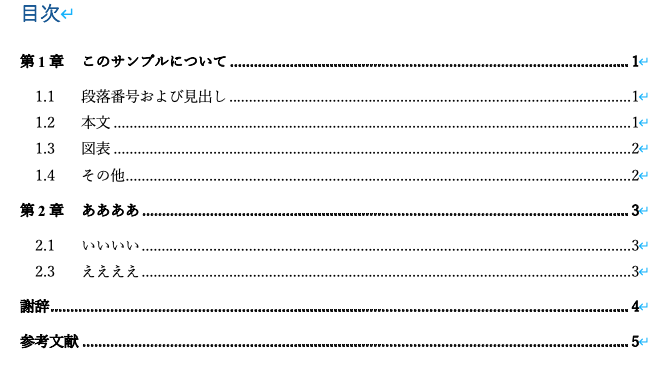
\includegraphics[width=.65\linewidth]{fig/fail-index.png}
  }
  \caption{目次の間違い}
  \label{fig:fail-index}
\end{figure}

\section{謝辞}

謝辞が祝辞だった(\figref{fig:fail-ack})。信じられないかもしれないけれど、本当にあった(確か2005年度)。

\begin{figure}[H]
    \centering
    \fbox{
        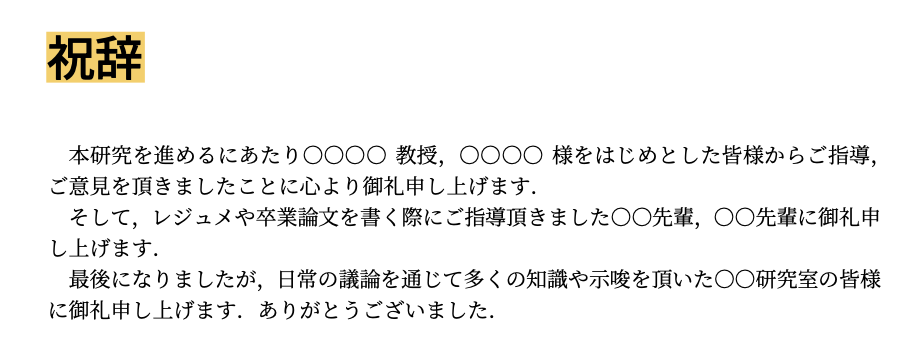
\includegraphics[width=.6\linewidth]{fig/fail-ack.png}
    }
    \caption{祝いの言葉}
    \label{fig:fail-ack}
\end{figure}  % 第5章
\chapter{結論}


% 本論文では○○○に着目し、△△△△アルゴリズムを提案した。シミュレーションの結果、
% 提案手法は条件Aにおいて従来手法に比べて$x$ \% 高速に動作することを確認した。
% 本手法は・・・・


% %%%%%%%%%%%%%%%%%%%%%%%%%%%%%%%%%%%%%%%%%%%%%%%%%%%%%%%%%%%%%%%%%%%%%%%
% \begin{comment}
%     \textblockcolour{pink}
%     \begin{textblock}{4}(16, 1)
%         【5】本文はここまで
%     \end{textblock}
    
%     \begin{textblock}{7}(11, 28)
%         本文は20ページ以上を目安とする。
%     \end{textblock}
% \end{comment}
% %%%%%%%%%%%%%%%%%%%%%%%%%%%%%%%%%%%%%%%%%%%%%%%%%%%%%%%%%%%%%%%%%%%%%%%
    % 第6章
% 謝辞
\theacknowledgments

%%%%%%%%%%%%%%%%%%%%%%%%%%%%%%%%%%%%%%%%%%%%%%%%%%%%%%%%%%%%%%%%%%%%%%%

\begin{comment}
    \textblockcolour{lime}
    \begin{textblock}{12}(6, 6)
        謝辞はなくてもよい。
        
        謝辞・参考文献・ソースコードなどの付録は本文に含まれない。
    \end{textblock}
    
    \begin{textblock}{12}(6, 12)
        論文全体で句読点の形式を統一する。
    
        このサンプルでは謝辞の句読点が他の章のそれと異なっている。
    
        どの句読点形式で執筆をするか指導教員に確認すること。
    \end{textblock}
\end{comment}
%%%%%%%%%%%%%%%%%%%%%%%%%%%%%%%%%%%%%%%%%%%%%%%%%%%%%%%%%%%%%%%%%%%%%%%

本研究を進めるにあたり○○○○ 教授,○○○○ 様をはじめとした皆様からご指導,ご意見を頂きましたことに心より御礼申し上げます.

そして,レジュメや卒業論文を書く際にご指導頂きました○○先輩,○○先輩に御礼申し上げます.

最後になりましたが,日常の議論を通じて多くの知識や示唆を頂いた○○研究室の皆様に御礼申し上げます.ありがとうございました.
         % 謝辞
% 参考文献
\bibliographystyle{junsrt}      % bibTexのスタイル
\bibliography{mybib}            % bibの読み込み

%%%%%%%%%%%%%%%%%%%%%%%%%%%%%%%%%%%%%%%%%%%%%%%%%%%%%%%%%%%%%%%%%%%%%%%

\begin{comment}
    \begin{textblock}{10}(7, 6)
      本文中で参照をした文献だけを載せる
    
      (本文中で参照していない文献を載せない)
    \end{textblock}
    
    \begin{textblock}{8}(11, 9.1)
      ←Webページはアクセス日時を記載する
    \end{textblock}
\end{comment}
%%%%%%%%%%%%%%%%%%%%%%%%%%%%%%%%%%%%%%%%%%%%%%%%%%%%%%%%%%%%%%%%%%%%%%%

% 英語と日本語の参考文献が混在することを考慮してbiblatexは利用しない
% \printbibliography% 参考文献

%\input{appendix}   % 付録
\end{document}
